\documentclass[1p]{elsarticle_modified}
%\bibliographystyle{elsarticle-num}

%\usepackage[colorlinks]{hyperref}
%\usepackage{abbrmath_seonhwa} %\Abb, \Ascr, \Acal ,\Abf, \Afrak
\usepackage{amsfonts}
\usepackage{amssymb}
\usepackage{amsmath}
\usepackage{amsthm}
\usepackage{scalefnt}
\usepackage{amsbsy}
\usepackage{kotex}
\usepackage{caption}
\usepackage{subfig}
\usepackage{color}
\usepackage{graphicx}
\usepackage{xcolor} %% white, black, red, green, blue, cyan, magenta, yellow
\usepackage{float}
\usepackage{setspace}
\usepackage{hyperref}

\usepackage{tikz}
\usetikzlibrary{arrows}

\usepackage{multirow}
\usepackage{array} % fixed length table
\usepackage{hhline}

%%%%%%%%%%%%%%%%%%%%%
\makeatletter
\renewcommand*\env@matrix[1][\arraystretch]{%
	\edef\arraystretch{#1}%
	\hskip -\arraycolsep
	\let\@ifnextchar\new@ifnextchar
	\array{*\c@MaxMatrixCols c}}
\makeatother %https://tex.stackexchange.com/questions/14071/how-can-i-increase-the-line-spacing-in-a-matrix
%%%%%%%%%%%%%%%

\usepackage[normalem]{ulem}

\newcommand{\msout}[1]{\ifmmode\text{\sout{\ensuremath{#1}}}\else\sout{#1}\fi}
%SOURCE: \msout is \stkout macro in https://tex.stackexchange.com/questions/20609/strikeout-in-math-mode

\newcommand{\cancel}[1]{
	\ifmmode
	{\color{red}\msout{#1}}
	\else
	{\color{red}\sout{#1}}
	\fi
}

\newcommand{\add}[1]{
	{\color{blue}\uwave{#1}}
}

\newcommand{\replace}[2]{
	\ifmmode
	{\color{red}\msout{#1}}{\color{blue}\uwave{#2}}
	\else
	{\color{red}\sout{#1}}{\color{blue}\uwave{#2}}
	\fi
}

\newcommand{\Sol}{\mathcal{S}} %segment
\newcommand{\D}{D} %diagram
\newcommand{\A}{\mathcal{A}} %arc


%%%%%%%%%%%%%%%%%%%%%%%%%%%%%5 test

\def\sl{\operatorname{\textup{SL}}(2,\Cbb)}
\def\psl{\operatorname{\textup{PSL}}(2,\Cbb)}
\def\quan{\mkern 1mu \triangleright \mkern 1mu}

\theoremstyle{definition}
\newtheorem{thm}{Theorem}[section]
\newtheorem{prop}[thm]{Proposition}
\newtheorem{lem}[thm]{Lemma}
\newtheorem{ques}[thm]{Question}
\newtheorem{cor}[thm]{Corollary}
\newtheorem{defn}[thm]{Definition}
\newtheorem{exam}[thm]{Example}
\newtheorem{rmk}[thm]{Remark}
\newtheorem{alg}[thm]{Algorithm}

\newcommand{\I}{\sqrt{-1}}
\begin{document}

%\begin{frontmatter}
%
%\title{Boundary parabolic representations of knots up to 8 crossings}
%
%%% Group authors per affiliation:
%\author{Yunhi Cho} 
%\address{Department of Mathematics, University of Seoul, Seoul, Korea}
%\ead{yhcho@uos.ac.kr}
%
%
%\author{Seonhwa Kim} %\fnref{s_kim}}
%\address{Center for Geometry and Physics, Institute for Basic Science, Pohang, 37673, Korea}
%\ead{ryeona17@ibs.re.kr}
%
%\author{Hyuk Kim}
%\address{Department of Mathematical Sciences, Seoul National University, Seoul 08826, Korea}
%\ead{hyukkim@snu.ac.kr}
%
%\author{Seokbeom Yoon}
%\address{Department of Mathematical Sciences, Seoul National University, Seoul, 08826,  Korea}
%\ead{sbyoon15@snu.ac.kr}
%
%\begin{abstract}
%We find all boundary parabolic representation of knots up to 8 crossings.
%
%\end{abstract}
%\begin{keyword}
%    \MSC[2010] 57M25 
%\end{keyword}
%
%\end{frontmatter}

%\linenumbers
%\tableofcontents
%
\newcommand\colored[1]{\textcolor{white}{\rule[-0.35ex]{0.8em}{1.4ex}}\kern-0.8em\color{red} #1}%
%\newcommand\colored[1]{\textcolor{white}{ #1}\kern-2.17ex	\textcolor{white}{ #1}\kern-1.81ex	\textcolor{white}{ #1}\kern-2.15ex\color{red}#1	}

{\Large $\underline{12n_{0479}~(K12n_{0479})}$}

\setlength{\tabcolsep}{10pt}
\renewcommand{\arraystretch}{1.6}
\vspace{1cm}\begin{tabular}{m{100pt}>{\centering\arraybackslash}m{274pt}}
\multirow{5}{120pt}{
	\centering
	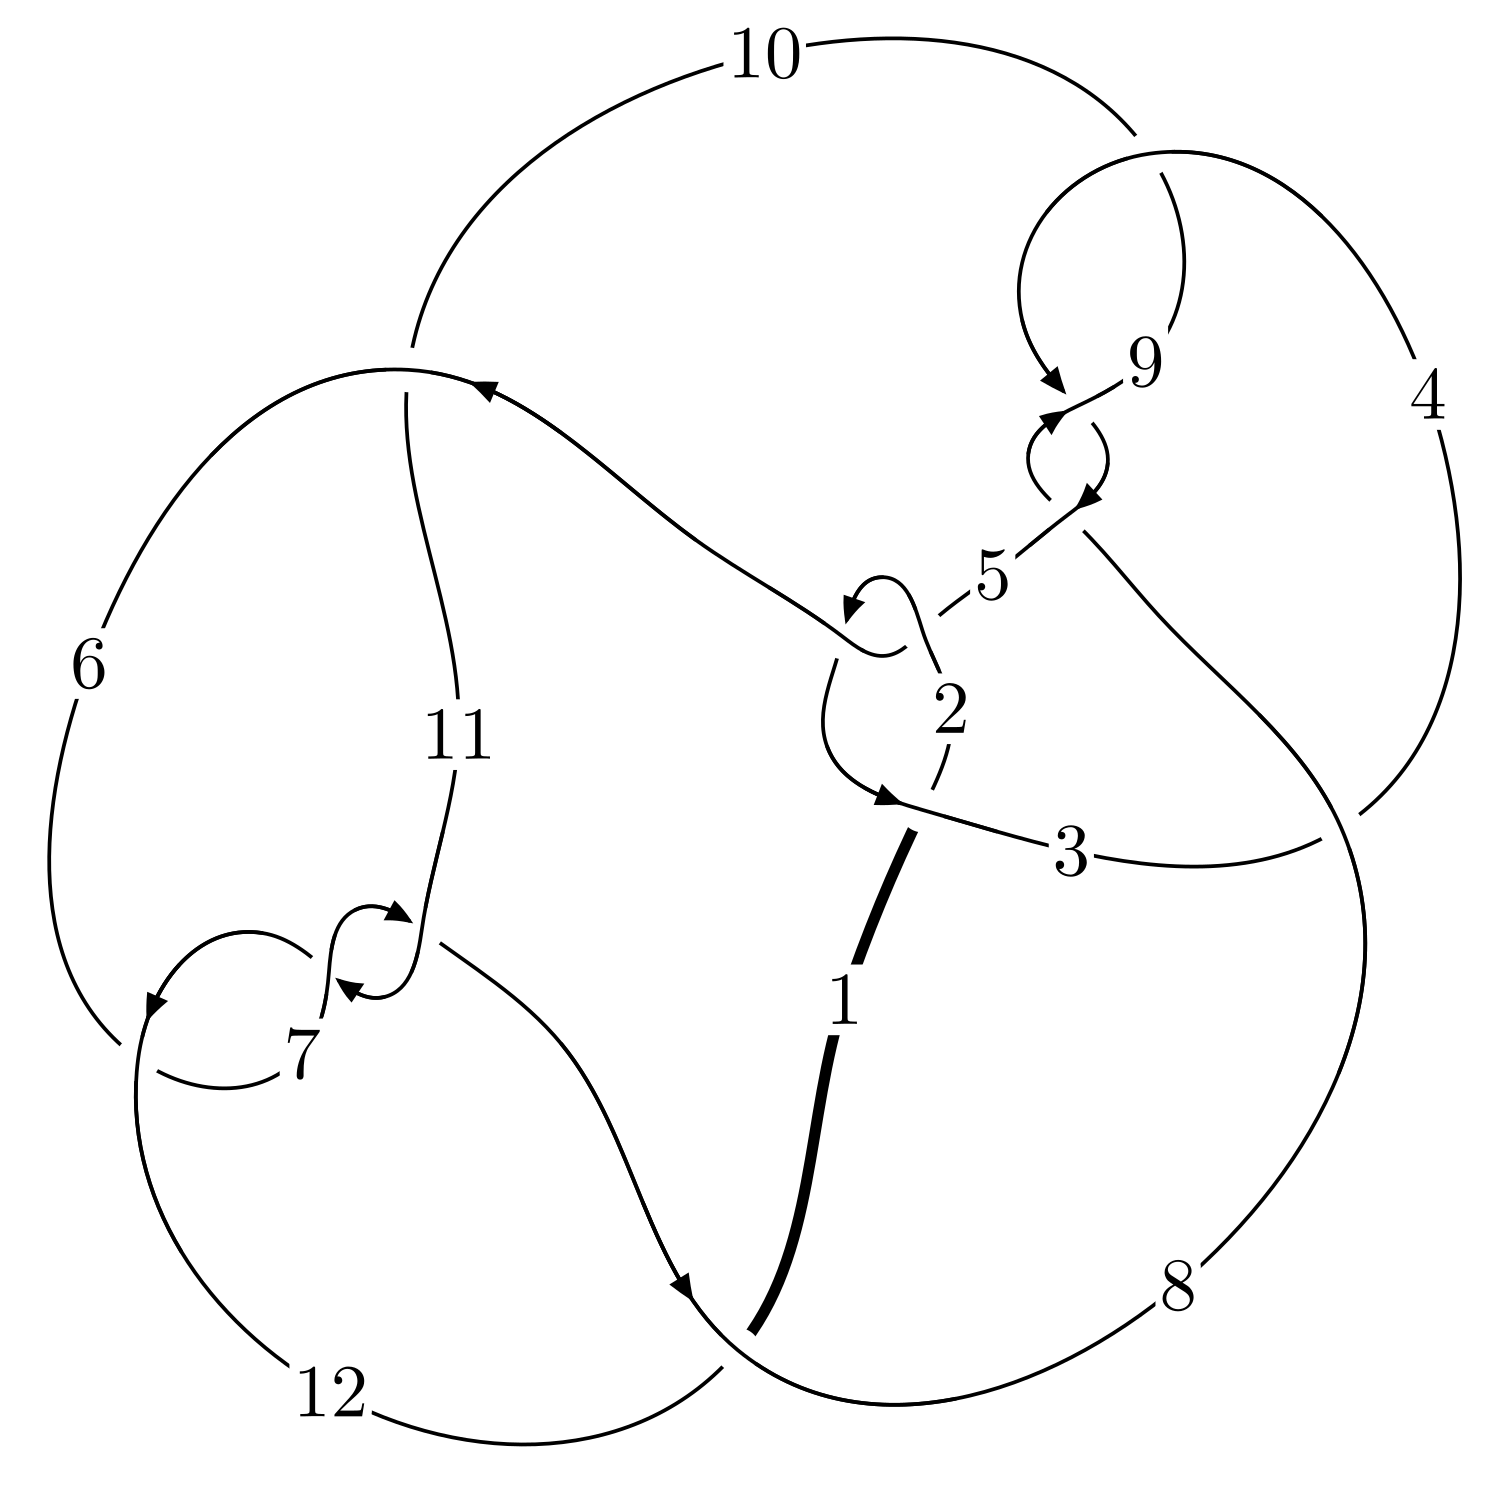
\includegraphics[width=112pt]{../../../GIT/diagram.site/Diagrams/png/2568_12n_0479.png}\\
\ \ \ A knot diagram\footnotemark}&
\allowdisplaybreaks
\textbf{Linearized knot diagam} \\
\cline{2-2}
 &
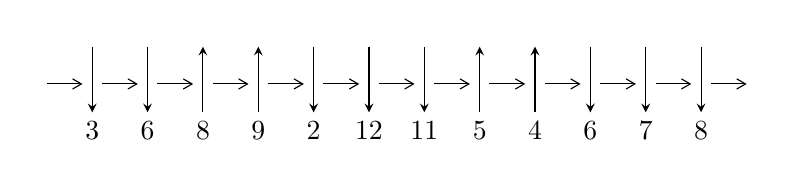
\begin{tikzpicture}[x=20pt, y=17pt]
	% nodes
	\node (C0) at (0, 0) {};
	\node (C1) at (1, 0) {};
	\node (C1U) at (1, +1) {};
	\node (C1D) at (1, -1) {3};

	\node (C2) at (2, 0) {};
	\node (C2U) at (2, +1) {};
	\node (C2D) at (2, -1) {6};

	\node (C3) at (3, 0) {};
	\node (C3U) at (3, +1) {};
	\node (C3D) at (3, -1) {8};

	\node (C4) at (4, 0) {};
	\node (C4U) at (4, +1) {};
	\node (C4D) at (4, -1) {9};

	\node (C5) at (5, 0) {};
	\node (C5U) at (5, +1) {};
	\node (C5D) at (5, -1) {2};

	\node (C6) at (6, 0) {};
	\node (C6U) at (6, +1) {};
	\node (C6D) at (6, -1) {12};

	\node (C7) at (7, 0) {};
	\node (C7U) at (7, +1) {};
	\node (C7D) at (7, -1) {11};

	\node (C8) at (8, 0) {};
	\node (C8U) at (8, +1) {};
	\node (C8D) at (8, -1) {5};

	\node (C9) at (9, 0) {};
	\node (C9U) at (9, +1) {};
	\node (C9D) at (9, -1) {4};

	\node (C10) at (10, 0) {};
	\node (C10U) at (10, +1) {};
	\node (C10D) at (10, -1) {6};

	\node (C11) at (11, 0) {};
	\node (C11U) at (11, +1) {};
	\node (C11D) at (11, -1) {7};

	\node (C12) at (12, 0) {};
	\node (C12U) at (12, +1) {};
	\node (C12D) at (12, -1) {8};
	\node (C13) at (13, 0) {};

	% arrows
	\draw[->,>={angle 60}]
	(C0) edge (C1) (C1) edge (C2) (C2) edge (C3) (C3) edge (C4) (C4) edge (C5) (C5) edge (C6) (C6) edge (C7) (C7) edge (C8) (C8) edge (C9) (C9) edge (C10) (C10) edge (C11) (C11) edge (C12) (C12) edge (C13) ;	\draw[->,>=stealth]
	(C1U) edge (C1D) (C2U) edge (C2D) (C3D) edge (C3U) (C4D) edge (C4U) (C5U) edge (C5D) (C6U) edge (C6D) (C7U) edge (C7D) (C8D) edge (C8U) (C9D) edge (C9U) (C10U) edge (C10D) (C11U) edge (C11D) (C12U) edge (C12D) ;
	\end{tikzpicture} \\
\hhline{~~} \\& 
\textbf{Solving Sequence} \\ \cline{2-2} 
 &
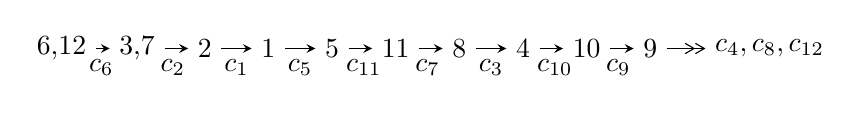
\begin{tikzpicture}[x=23pt, y=7pt]
	% node
	\node (A0) at (-1/8, 0) {6,12};
	\node (A1) at (17/16, 0) {3,7};
	\node (A2) at (17/8, 0) {2};
	\node (A3) at (25/8, 0) {1};
	\node (A4) at (33/8, 0) {5};
	\node (A5) at (41/8, 0) {11};
	\node (A6) at (49/8, 0) {8};
	\node (A7) at (57/8, 0) {4};
	\node (A8) at (65/8, 0) {10};
	\node (A9) at (73/8, 0) {9};
	\node (C1) at (1/2, -1) {$c_{6}$};
	\node (C2) at (13/8, -1) {$c_{2}$};
	\node (C3) at (21/8, -1) {$c_{1}$};
	\node (C4) at (29/8, -1) {$c_{5}$};
	\node (C5) at (37/8, -1) {$c_{11}$};
	\node (C6) at (45/8, -1) {$c_{7}$};
	\node (C7) at (53/8, -1) {$c_{3}$};
	\node (C8) at (61/8, -1) {$c_{10}$};
	\node (C9) at (69/8, -1) {$c_{9}$};
	\node (A10) at (11, 0) {$c_{4},c_{8},c_{12}$};

	% edge
	\draw[->,>=stealth]	
	(A0) edge (A1) (A1) edge (A2) (A2) edge (A3) (A3) edge (A4) (A4) edge (A5) (A5) edge (A6) (A6) edge (A7) (A7) edge (A8) (A8) edge (A9) ;
	\draw[->>,>={angle 60}]	
	(A9) edge (A10);
\end{tikzpicture} \\ 

\end{tabular} \\

\footnotetext{
The image of knot diagram is generated by the software ``\textbf{Draw programme}" developed by Andrew Bartholomew(\url{http://www.layer8.co.uk/maths/draw/index.htm\#Running-draw}), where we modified some parts for our purpose(\url{https://github.com/CATsTAILs/LinksPainter}).
}\phantom \\ \newline 
\centering \textbf{Ideals for irreducible components\footnotemark of $X_{\text{par}}$} 
 
\begin{align*}
I^u_{1}&=\langle 
186488768414913 u^{49}-290002817250832 u^{48}+\cdots+308976956670931 b+23795142626938,\\
\phantom{I^u_{1}}&\phantom{= \langle  }-2.98208\times10^{14} u^{49}+1.16633\times10^{15} u^{48}+\cdots+1.85386\times10^{15} a-3.97700\times10^{15},\;u^{50}-2 u^{49}+\cdots+7 u-3\rangle \\
I^u_{2}&=\langle 
b-1,\;-2 u^2 a+a^2-2 a u+4 u^2-4 a+3 u+7,\;u^3+u^2+2 u+1\rangle \\
I^u_{3}&=\langle 
b+1,\;u^2+a- u+2,\;u^3- u^2+2 u-1\rangle \\
\\
\end{align*}
\raggedright * 3 irreducible components of $\dim_{\mathbb{C}}=0$, with total 59 representations.\\
\footnotetext{All coefficients of polynomials are rational numbers. But the coefficients are sometimes approximated in decimal forms when there is not enough margin.}
\newpage
\renewcommand{\arraystretch}{1}
\centering \section*{I. $I^u_{1}= \langle 1.86\times10^{14} u^{49}-2.90\times10^{14} u^{48}+\cdots+3.09\times10^{14} b+2.38\times10^{13},\;-2.98\times10^{14} u^{49}+1.17\times10^{15} u^{48}+\cdots+1.85\times10^{15} a-3.98\times10^{15},\;u^{50}-2 u^{49}+\cdots+7 u-3 \rangle$}
\flushleft \textbf{(i) Arc colorings}\\
\begin{tabular}{m{7pt} m{180pt} m{7pt} m{180pt} }
\flushright $a_{6}=$&$\begin{pmatrix}1\\0\end{pmatrix}$ \\
\flushright $a_{12}=$&$\begin{pmatrix}0\\u\end{pmatrix}$ \\
\flushright $a_{3}=$&$\begin{pmatrix}0.160858 u^{49}-0.629138 u^{48}+\cdots-4.21769 u+2.14525\\-0.603569 u^{49}+0.938590 u^{48}+\cdots+1.19866 u-0.0770127\end{pmatrix}$ \\
\flushright $a_{7}=$&$\begin{pmatrix}1\\u^2\end{pmatrix}$ \\
\flushright $a_{2}=$&$\begin{pmatrix}-0.442711 u^{49}+0.309453 u^{48}+\cdots-3.01903 u+2.06824\\-0.603569 u^{49}+0.938590 u^{48}+\cdots+1.19866 u-0.0770127\end{pmatrix}$ \\
\flushright $a_{1}=$&$\begin{pmatrix}- u^5-2 u^3- u\\- u^7-3 u^5-2 u^3+u\end{pmatrix}$ \\
\flushright $a_{5}=$&$\begin{pmatrix}-0.0498473 u^{49}-0.638746 u^{48}+\cdots+5.09518 u+0.739281\\-0.316393 u^{49}+0.485397 u^{48}+\cdots+2.60385 u-0.176830\end{pmatrix}$ \\
\flushright $a_{11}=$&$\begin{pmatrix}u\\u^3+u\end{pmatrix}$ \\
\flushright $a_{8}=$&$\begin{pmatrix}u^2+1\\u^4+2 u^2\end{pmatrix}$ \\
\flushright $a_{4}=$&$\begin{pmatrix}-0.0589435 u^{49}-0.198506 u^{48}+\cdots-4.62549 u+2.19124\\-0.738441 u^{49}+1.20164 u^{48}+\cdots+1.08821 u-0.149542\end{pmatrix}$ \\
\flushright $a_{10}=$&$\begin{pmatrix}u^3+2 u\\u^3+u\end{pmatrix}$ \\
\flushright $a_{9}=$&$\begin{pmatrix}0.660432 u^{49}-0.972483 u^{48}+\cdots-0.425785 u+2.52397\\0.348382 u^{49}-0.970681 u^{48}+\cdots-2.09905 u+1.98130\end{pmatrix}$\\&\end{tabular}
\flushleft \textbf{(ii) Obstruction class $= -1$}\\~\\
\flushleft \textbf{(iii) Cusp Shapes $= -\frac{818278759941418}{308976956670931} u^{49}+\frac{1283399787362471}{308976956670931} u^{48}+\cdots+\frac{3241957768122858}{308976956670931} u-\frac{3010107002943738}{308976956670931}$}\\~\\
\newpage\renewcommand{\arraystretch}{1}
\flushleft \textbf{(iv) u-Polynomials at the component}\newline \\
\begin{tabular}{m{50pt}|m{274pt}}
Crossings & \hspace{64pt}u-Polynomials at each crossing \\
\hline $$\begin{aligned}c_{1}\end{aligned}$$&$\begin{aligned}
&u^{50}+18 u^{49}+\cdots+4150 u+289
\end{aligned}$\\
\hline $$\begin{aligned}c_{2},c_{5}\end{aligned}$$&$\begin{aligned}
&u^{50}+4 u^{49}+\cdots-28 u-17
\end{aligned}$\\
\hline $$\begin{aligned}c_{3}\end{aligned}$$&$\begin{aligned}
&u^{50}+u^{49}+\cdots+1024 u+488
\end{aligned}$\\
\hline $$\begin{aligned}c_{4},c_{8},c_{9}\end{aligned}$$&$\begin{aligned}
&u^{50}- u^{49}+\cdots-16 u+8
\end{aligned}$\\
\hline $$\begin{aligned}c_{6},c_{7},c_{11}\end{aligned}$$&$\begin{aligned}
&u^{50}+2 u^{49}+\cdots-7 u-3
\end{aligned}$\\
\hline $$\begin{aligned}c_{10},c_{12}\end{aligned}$$&$\begin{aligned}
&u^{50}-2 u^{49}+\cdots-3995 u-2391
\end{aligned}$\\
\hline
\end{tabular}\\~\\
\newpage\renewcommand{\arraystretch}{1}
\flushleft \textbf{(v) Riley Polynomials at the component}\newline \\
\begin{tabular}{m{50pt}|m{274pt}}
Crossings & \hspace{64pt}Riley Polynomials at each crossing \\
\hline $$\begin{aligned}c_{1}\end{aligned}$$&$\begin{aligned}
&y^{50}+38 y^{49}+\cdots+3129458 y+83521
\end{aligned}$\\
\hline $$\begin{aligned}c_{2},c_{5}\end{aligned}$$&$\begin{aligned}
&y^{50}-18 y^{49}+\cdots-4150 y+289
\end{aligned}$\\
\hline $$\begin{aligned}c_{3}\end{aligned}$$&$\begin{aligned}
&y^{50}-41 y^{49}+\cdots-2344704 y+238144
\end{aligned}$\\
\hline $$\begin{aligned}c_{4},c_{8},c_{9}\end{aligned}$$&$\begin{aligned}
&y^{50}+43 y^{49}+\cdots-896 y+64
\end{aligned}$\\
\hline $$\begin{aligned}c_{6},c_{7},c_{11}\end{aligned}$$&$\begin{aligned}
&y^{50}+48 y^{49}+\cdots-79 y+9
\end{aligned}$\\
\hline $$\begin{aligned}c_{10},c_{12}\end{aligned}$$&$\begin{aligned}
&y^{50}+16 y^{49}+\cdots+33729737 y+5716881
\end{aligned}$\\
\hline
\end{tabular}\\~\\
\newpage\flushleft \textbf{(vi) Complex Volumes and Cusp Shapes}
$$\begin{array}{c|c|c}  
\text{Solutions to }I^u_{1}& \I (\text{vol} + \sqrt{-1}CS) & \text{Cusp shape}\\
 \hline 
\begin{aligned}
u &= \phantom{-}0.548026 + 0.636865 I \\
a &= -0.141399 + 0.209810 I \\
b &= \phantom{-}1.031990 - 0.770119 I\end{aligned}
 & \phantom{-}0.14665 + 5.50869 I & -5.48648 - 2.48413 I \\ \hline\begin{aligned}
u &= \phantom{-}0.548026 - 0.636865 I \\
a &= -0.141399 - 0.209810 I \\
b &= \phantom{-}1.031990 + 0.770119 I\end{aligned}
 & \phantom{-}0.14665 - 5.50869 I & -5.48648 + 2.48413 I \\ \hline\begin{aligned}
u &= \phantom{-}0.747661 + 0.370902 I \\
a &= \phantom{-}1.27766 - 1.31418 I \\
b &= \phantom{-}1.119580 + 0.753217 I\end{aligned}
 & -0.80164 - 9.94223 I & -7.39959 + 7.60109 I \\ \hline\begin{aligned}
u &= \phantom{-}0.747661 - 0.370902 I \\
a &= \phantom{-}1.27766 + 1.31418 I \\
b &= \phantom{-}1.119580 - 0.753217 I\end{aligned}
 & -0.80164 + 9.94223 I & -7.39959 - 7.60109 I \\ \hline\begin{aligned}
u &= -0.701764 + 0.430117 I \\
a &= -1.00242 - 1.23319 I \\
b &= -0.971275 + 0.823552 I\end{aligned}
 & \phantom{-}4.04082 + 5.32876 I & -2.84513 - 5.88571 I \\ \hline\begin{aligned}
u &= -0.701764 - 0.430117 I \\
a &= -1.00242 + 1.23319 I \\
b &= -0.971275 - 0.823552 I\end{aligned}
 & \phantom{-}4.04082 - 5.32876 I & -2.84513 + 5.88571 I \\ \hline\begin{aligned}
u &= -0.613532 + 0.535693 I \\
a &= \phantom{-}0.370473 + 0.106254 I \\
b &= -0.839697 - 0.858575 I\end{aligned}
 & \phantom{-}4.44373 - 0.93541 I & -1.58239 - 0.30026 I \\ \hline\begin{aligned}
u &= -0.613532 - 0.535693 I \\
a &= \phantom{-}0.370473 - 0.106254 I \\
b &= -0.839697 + 0.858575 I\end{aligned}
 & \phantom{-}4.44373 + 0.93541 I & -1.58239 + 0.30026 I \\ \hline\begin{aligned}
u &= \phantom{-}0.680028 + 0.435043 I \\
a &= -0.548393 - 0.018507 I \\
b &= \phantom{-}0.600139 - 0.934400 I\end{aligned}
 & \phantom{-}0.78344 - 3.70599 I & -5.05675 + 3.80006 I \\ \hline\begin{aligned}
u &= \phantom{-}0.680028 - 0.435043 I \\
a &= -0.548393 + 0.018507 I \\
b &= \phantom{-}0.600139 + 0.934400 I\end{aligned}
 & \phantom{-}0.78344 + 3.70599 I & -5.05675 - 3.80006 I\\
 \hline 
 \end{array}$$\newpage$$\begin{array}{c|c|c}  
\text{Solutions to }I^u_{1}& \I (\text{vol} + \sqrt{-1}CS) & \text{Cusp shape}\\
 \hline 
\begin{aligned}
u &= \phantom{-}0.609239 + 0.505071 I \\
a &= \phantom{-}0.659368 - 1.086520 I \\
b &= \phantom{-}0.728352 + 0.857268 I\end{aligned}
 & \phantom{-}1.077150 - 0.581801 I & -4.57087 + 2.28469 I \\ \hline\begin{aligned}
u &= \phantom{-}0.609239 - 0.505071 I \\
a &= \phantom{-}0.659368 + 1.086520 I \\
b &= \phantom{-}0.728352 - 0.857268 I\end{aligned}
 & \phantom{-}1.077150 + 0.581801 I & -4.57087 - 2.28469 I \\ \hline\begin{aligned}
u &= -0.314558 + 1.181770 I \\
a &= \phantom{-}0.755396 + 0.911108 I \\
b &= \phantom{-}0.883202 - 0.570553 I\end{aligned}
 & -1.86240 + 5.95457 I & \phantom{-0.000000 } 0 \\ \hline\begin{aligned}
u &= -0.314558 - 1.181770 I \\
a &= \phantom{-}0.755396 - 0.911108 I \\
b &= \phantom{-}0.883202 + 0.570553 I\end{aligned}
 & -1.86240 - 5.95457 I & \phantom{-0.000000 } 0 \\ \hline\begin{aligned}
u &= -0.754187 + 0.037133 I \\
a &= \phantom{-}1.177820 + 0.351943 I \\
b &= \phantom{-}0.791193 + 0.522358 I\end{aligned}
 & -5.37048 - 2.06528 I & -9.77366 + 3.43997 I \\ \hline\begin{aligned}
u &= -0.754187 - 0.037133 I \\
a &= \phantom{-}1.177820 - 0.351943 I \\
b &= \phantom{-}0.791193 - 0.522358 I\end{aligned}
 & -5.37048 + 2.06528 I & -9.77366 - 3.43997 I \\ \hline\begin{aligned}
u &= -0.030213 + 1.260010 I \\
a &= -0.22647 + 1.85610 I \\
b &= -1.111340 - 0.290888 I\end{aligned}
 & -3.90026 + 0.44346 I & \phantom{-0.000000 } 0 \\ \hline\begin{aligned}
u &= -0.030213 - 1.260010 I \\
a &= -0.22647 - 1.85610 I \\
b &= -1.111340 + 0.290888 I\end{aligned}
 & -3.90026 - 0.44346 I & \phantom{-0.000000 } 0 \\ \hline\begin{aligned}
u &= \phantom{-}0.251247 + 1.259910 I \\
a &= -0.547258 + 0.656638 I \\
b &= -0.684570 - 0.219108 I\end{aligned}
 & \phantom{-}2.05074 - 3.33048 I & \phantom{-0.000000 } 0 \\ \hline\begin{aligned}
u &= \phantom{-}0.251247 - 1.259910 I \\
a &= -0.547258 - 0.656638 I \\
b &= -0.684570 + 0.219108 I\end{aligned}
 & \phantom{-}2.05074 + 3.33048 I & \phantom{-0.000000 } 0\\
 \hline 
 \end{array}$$\newpage$$\begin{array}{c|c|c}  
\text{Solutions to }I^u_{1}& \I (\text{vol} + \sqrt{-1}CS) & \text{Cusp shape}\\
 \hline 
\begin{aligned}
u &= -0.299311 + 1.263120 I \\
a &= \phantom{-}0.021398 + 0.222536 I \\
b &= \phantom{-}0.705583 + 0.479463 I\end{aligned}
 & -1.35085 + 1.74111 I & \phantom{-0.000000 } 0 \\ \hline\begin{aligned}
u &= -0.299311 - 1.263120 I \\
a &= \phantom{-}0.021398 - 0.222536 I \\
b &= \phantom{-}0.705583 - 0.479463 I\end{aligned}
 & -1.35085 - 1.74111 I & \phantom{-0.000000 } 0 \\ \hline\begin{aligned}
u &= -0.095422 + 1.324880 I \\
a &= -0.023038 + 1.203270 I \\
b &= \phantom{-}1.169140 - 0.223723 I\end{aligned}
 & \phantom{-}1.85552 + 1.71056 I & \phantom{-0.000000 } 0 \\ \hline\begin{aligned}
u &= -0.095422 - 1.324880 I \\
a &= -0.023038 - 1.203270 I \\
b &= \phantom{-}1.169140 + 0.223723 I\end{aligned}
 & \phantom{-}1.85552 - 1.71056 I & \phantom{-0.000000 } 0 \\ \hline\begin{aligned}
u &= \phantom{-}0.667644\phantom{ +0.000000I} \\
a &= -1.23502\phantom{ +0.000000I} \\
b &= -0.589141\phantom{ +0.000000I}\end{aligned}
 & -1.84778\phantom{ +0.000000I} & -2.14880\phantom{ +0.000000I} \\ \hline\begin{aligned}
u &= -0.179331 + 1.371620 I \\
a &= \phantom{-}1.20289 - 1.64393 I \\
b &= -0.538230 + 0.405630 I\end{aligned}
 & -1.78664 + 3.49510 I & \phantom{-0.000000 } 0 \\ \hline\begin{aligned}
u &= -0.179331 - 1.371620 I \\
a &= \phantom{-}1.20289 + 1.64393 I \\
b &= -0.538230 - 0.405630 I\end{aligned}
 & -1.78664 - 3.49510 I & \phantom{-0.000000 } 0 \\ \hline\begin{aligned}
u &= \phantom{-}0.523052 + 0.312664 I \\
a &= -1.58769 + 0.98505 I \\
b &= -1.278040 + 0.059074 I\end{aligned}
 & -5.97365 - 1.50019 I & -9.06126 + 4.58058 I \\ \hline\begin{aligned}
u &= \phantom{-}0.523052 - 0.312664 I \\
a &= -1.58769 - 0.98505 I \\
b &= -1.278040 - 0.059074 I\end{aligned}
 & -5.97365 + 1.50019 I & -9.06126 - 4.58058 I \\ \hline\begin{aligned}
u &= \phantom{-}0.062298 + 1.409670 I \\
a &= -0.212165 - 1.347970 I \\
b &= \phantom{-}0.181198 + 0.793511 I\end{aligned}
 & \phantom{-}5.34369 - 2.04364 I & \phantom{-0.000000 } 0\\
 \hline 
 \end{array}$$\newpage$$\begin{array}{c|c|c}  
\text{Solutions to }I^u_{1}& \I (\text{vol} + \sqrt{-1}CS) & \text{Cusp shape}\\
 \hline 
\begin{aligned}
u &= \phantom{-}0.062298 - 1.409670 I \\
a &= -0.212165 + 1.347970 I \\
b &= \phantom{-}0.181198 - 0.793511 I\end{aligned}
 & \phantom{-}5.34369 + 2.04364 I & \phantom{-0.000000 } 0 \\ \hline\begin{aligned}
u &= \phantom{-}0.20226 + 1.41029 I \\
a &= \phantom{-}0.244900 + 0.806956 I \\
b &= -1.348940 + 0.042324 I\end{aligned}
 & -0.46882 - 4.20038 I & \phantom{-0.000000 } 0 \\ \hline\begin{aligned}
u &= \phantom{-}0.20226 - 1.41029 I \\
a &= \phantom{-}0.244900 - 0.806956 I \\
b &= -1.348940 - 0.042324 I\end{aligned}
 & -0.46882 + 4.20038 I & \phantom{-0.000000 } 0 \\ \hline\begin{aligned}
u &= -0.478945 + 0.205762 I \\
a &= \phantom{-}1.01707 - 2.37277 I \\
b &= -0.767299 + 0.234309 I\end{aligned}
 & -6.81379 + 1.04376 I & -7.43326 - 6.78776 I \\ \hline\begin{aligned}
u &= -0.478945 - 0.205762 I \\
a &= \phantom{-}1.01707 + 2.37277 I \\
b &= -0.767299 - 0.234309 I\end{aligned}
 & -6.81379 - 1.04376 I & -7.43326 + 6.78776 I \\ \hline\begin{aligned}
u &= \phantom{-}0.28571 + 1.46065 I \\
a &= \phantom{-}0.22222 - 2.14370 I \\
b &= \phantom{-}1.175840 + 0.774815 I\end{aligned}
 & \phantom{-}5.0883 - 13.7071 I & \phantom{-0.000000 } 0 \\ \hline\begin{aligned}
u &= \phantom{-}0.28571 - 1.46065 I \\
a &= \phantom{-}0.22222 + 2.14370 I \\
b &= \phantom{-}1.175840 - 0.774815 I\end{aligned}
 & \phantom{-}5.0883 + 13.7071 I & \phantom{-0.000000 } 0 \\ \hline\begin{aligned}
u &= \phantom{-}0.24689 + 1.47668 I \\
a &= -1.12288 + 0.98727 I \\
b &= \phantom{-}0.577120 - 1.045150 I\end{aligned}
 & \phantom{-}6.96288 - 7.09069 I & \phantom{-0.000000 } 0 \\ \hline\begin{aligned}
u &= \phantom{-}0.24689 - 1.47668 I \\
a &= -1.12288 - 0.98727 I \\
b &= \phantom{-}0.577120 + 1.045150 I\end{aligned}
 & \phantom{-}6.96288 + 7.09069 I & \phantom{-0.000000 } 0 \\ \hline\begin{aligned}
u &= \phantom{-}0.21123 + 1.48331 I \\
a &= -0.10979 - 1.94214 I \\
b &= \phantom{-}0.854567 + 0.927257 I\end{aligned}
 & \phantom{-}7.49634 - 3.56090 I & \phantom{-0.000000 } 0\\
 \hline 
 \end{array}$$\newpage$$\begin{array}{c|c|c}  
\text{Solutions to }I^u_{1}& \I (\text{vol} + \sqrt{-1}CS) & \text{Cusp shape}\\
 \hline 
\begin{aligned}
u &= \phantom{-}0.21123 - 1.48331 I \\
a &= -0.10979 + 1.94214 I \\
b &= \phantom{-}0.854567 - 0.927257 I\end{aligned}
 & \phantom{-}7.49634 + 3.56090 I & \phantom{-0.000000 } 0 \\ \hline\begin{aligned}
u &= -0.25705 + 1.47829 I \\
a &= -0.06564 - 2.05483 I \\
b &= -1.058610 + 0.870913 I\end{aligned}
 & \phantom{-}10.20760 + 8.82997 I & \phantom{-0.000000 } 0 \\ \hline\begin{aligned}
u &= -0.25705 - 1.47829 I \\
a &= -0.06564 + 2.05483 I \\
b &= -1.058610 - 0.870913 I\end{aligned}
 & \phantom{-}10.20760 - 8.82997 I & \phantom{-0.000000 } 0 \\ \hline\begin{aligned}
u &= \phantom{-}0.15233 + 1.49913 I \\
a &= -1.01986 + 1.15371 I \\
b &= \phantom{-}0.992952 - 0.891101 I\end{aligned}
 & \phantom{-}7.08236 + 3.11695 I & \phantom{-0.000000 } 0 \\ \hline\begin{aligned}
u &= \phantom{-}0.15233 - 1.49913 I \\
a &= -1.01986 - 1.15371 I \\
b &= \phantom{-}0.992952 + 0.891101 I\end{aligned}
 & \phantom{-}7.08236 - 3.11695 I & \phantom{-0.000000 } 0 \\ \hline\begin{aligned}
u &= -0.20291 + 1.49495 I \\
a &= \phantom{-}1.08852 + 1.06865 I \\
b &= -0.799853 - 0.997275 I\end{aligned}
 & \phantom{-}11.03000 + 2.01018 I & \phantom{-0.000000 } 0 \\ \hline\begin{aligned}
u &= -0.20291 - 1.49495 I \\
a &= \phantom{-}1.08852 - 1.06865 I \\
b &= -0.799853 + 0.997275 I\end{aligned}
 & \phantom{-}11.03000 - 2.01018 I & \phantom{-0.000000 } 0 \\ \hline\begin{aligned}
u &= \phantom{-}0.275380 + 0.327909 I \\
a &= -0.267865 - 0.801075 I \\
b &= \phantom{-}0.330232 + 0.361285 I\end{aligned}
 & -0.199328 - 0.932041 I & -3.89641 + 7.43641 I \\ \hline\begin{aligned}
u &= \phantom{-}0.275380 - 0.327909 I \\
a &= -0.267865 + 0.801075 I \\
b &= \phantom{-}0.330232 - 0.361285 I\end{aligned}
 & -0.199328 + 0.932041 I & -3.89641 - 7.43641 I \\ \hline\begin{aligned}
u &= -0.403899\phantom{ +0.000000I} \\
a &= \phantom{-}2.57601\phantom{ +0.000000I} \\
b &= \phantom{-}1.10270\phantom{ +0.000000I}\end{aligned}
 & -2.29285\phantom{ +0.000000I} & \phantom{-}3.34720\phantom{ +0.000000I}\\
 \hline 
 \end{array}$$\newpage\newpage\renewcommand{\arraystretch}{1}
\centering \section*{II. $I^u_{2}= \langle b-1,\;-2 u^2 a+a^2-2 a u+4 u^2-4 a+3 u+7,\;u^3+u^2+2 u+1 \rangle$}
\flushleft \textbf{(i) Arc colorings}\\
\begin{tabular}{m{7pt} m{180pt} m{7pt} m{180pt} }
\flushright $a_{6}=$&$\begin{pmatrix}1\\0\end{pmatrix}$ \\
\flushright $a_{12}=$&$\begin{pmatrix}0\\u\end{pmatrix}$ \\
\flushright $a_{3}=$&$\begin{pmatrix}a\\1\end{pmatrix}$ \\
\flushright $a_{7}=$&$\begin{pmatrix}1\\u^2\end{pmatrix}$ \\
\flushright $a_{2}=$&$\begin{pmatrix}a+1\\1\end{pmatrix}$ \\
\flushright $a_{1}=$&$\begin{pmatrix}1\\0\end{pmatrix}$ \\
\flushright $a_{5}=$&$\begin{pmatrix}- a\\-1\end{pmatrix}$ \\
\flushright $a_{11}=$&$\begin{pmatrix}u\\- u^2- u-1\end{pmatrix}$ \\
\flushright $a_{8}=$&$\begin{pmatrix}u^2+1\\u^2+u+1\end{pmatrix}$ \\
\flushright $a_{4}=$&$\begin{pmatrix}u^2+u+2\\a u+2\end{pmatrix}$ \\
\flushright $a_{10}=$&$\begin{pmatrix}- u^2-1\\- u^2- u-1\end{pmatrix}$ \\
\flushright $a_{9}=$&$\begin{pmatrix}u^2 a-2 u^2+a-3\\u^2 a+a u+a+u\end{pmatrix}$\\&\end{tabular}
\flushleft \textbf{(ii) Obstruction class $= 1$}\\~\\
\flushleft \textbf{(iii) Cusp Shapes $= -4 u^2-4 u-16$}\\~\\
\newpage\renewcommand{\arraystretch}{1}
\flushleft \textbf{(iv) u-Polynomials at the component}\newline \\
\begin{tabular}{m{50pt}|m{274pt}}
Crossings & \hspace{64pt}u-Polynomials at each crossing \\
\hline $$\begin{aligned}c_{1},c_{5}\end{aligned}$$&$\begin{aligned}
&(u-1)^6
\end{aligned}$\\
\hline $$\begin{aligned}c_{2}\end{aligned}$$&$\begin{aligned}
&(u+1)^6
\end{aligned}$\\
\hline $$\begin{aligned}c_{3},c_{4},c_{8}\\c_{9}\end{aligned}$$&$\begin{aligned}
&(u^2+2)^3
\end{aligned}$\\
\hline $$\begin{aligned}c_{6},c_{7}\end{aligned}$$&$\begin{aligned}
&(u^3+u^2+2 u+1)^2
\end{aligned}$\\
\hline $$\begin{aligned}c_{10},c_{12}\end{aligned}$$&$\begin{aligned}
&(u^3+u^2-1)^2
\end{aligned}$\\
\hline $$\begin{aligned}c_{11}\end{aligned}$$&$\begin{aligned}
&(u^3- u^2+2 u-1)^2
\end{aligned}$\\
\hline
\end{tabular}\\~\\
\newpage\renewcommand{\arraystretch}{1}
\flushleft \textbf{(v) Riley Polynomials at the component}\newline \\
\begin{tabular}{m{50pt}|m{274pt}}
Crossings & \hspace{64pt}Riley Polynomials at each crossing \\
\hline $$\begin{aligned}c_{1},c_{2},c_{5}\end{aligned}$$&$\begin{aligned}
&(y-1)^6
\end{aligned}$\\
\hline $$\begin{aligned}c_{3},c_{4},c_{8}\\c_{9}\end{aligned}$$&$\begin{aligned}
&(y+2)^6
\end{aligned}$\\
\hline $$\begin{aligned}c_{6},c_{7},c_{11}\end{aligned}$$&$\begin{aligned}
&(y^3+3 y^2+2 y-1)^2
\end{aligned}$\\
\hline $$\begin{aligned}c_{10},c_{12}\end{aligned}$$&$\begin{aligned}
&(y^3- y^2+2 y-1)^2
\end{aligned}$\\
\hline
\end{tabular}\\~\\
\newpage\flushleft \textbf{(vi) Complex Volumes and Cusp Shapes}
$$\begin{array}{c|c|c}  
\text{Solutions to }I^u_{2}& \I (\text{vol} + \sqrt{-1}CS) & \text{Cusp shape}\\
 \hline 
\begin{aligned}
u &= -0.215080 + 1.307140 I \\
a &= \phantom{-}0.917744 - 0.191855 I \\
b &= \phantom{-}1.00000\phantom{ +0.000000I}\end{aligned}
 & -3.55561 + 2.82812 I & -8.49024 - 2.97945 I \\ \hline\begin{aligned}
u &= -0.215080 + 1.307140 I \\
a &= -0.67262 + 1.68158 I \\
b &= \phantom{-}1.00000\phantom{ +0.000000I}\end{aligned}
 & -3.55561 + 2.82812 I & -8.49024 - 2.97945 I \\ \hline\begin{aligned}
u &= -0.215080 - 1.307140 I \\
a &= \phantom{-}0.917744 + 0.191855 I \\
b &= \phantom{-}1.00000\phantom{ +0.000000I}\end{aligned}
 & -3.55561 - 2.82812 I & -8.49024 + 2.97945 I \\ \hline\begin{aligned}
u &= -0.215080 - 1.307140 I \\
a &= -0.67262 - 1.68158 I \\
b &= \phantom{-}1.00000\phantom{ +0.000000I}\end{aligned}
 & -3.55561 - 2.82812 I & -8.49024 + 2.97945 I \\ \hline\begin{aligned}
u &= -0.569840\phantom{ +0.000000I} \\
a &= \phantom{-}1.75488 + 1.87343 I \\
b &= \phantom{-}1.00000\phantom{ +0.000000I}\end{aligned}
 & -7.69319\phantom{ +0.000000I} & -15.0200\phantom{ +0.000000I} \\ \hline\begin{aligned}
u &= -0.569840\phantom{ +0.000000I} \\
a &= \phantom{-}1.75488 - 1.87343 I \\
b &= \phantom{-}1.00000\phantom{ +0.000000I}\end{aligned}
 & -7.69319\phantom{ +0.000000I} & -15.0200\phantom{ +0.000000I}\\
 \hline 
 \end{array}$$\newpage\newpage\renewcommand{\arraystretch}{1}
\centering \section*{III. $I^u_{3}= \langle b+1,\;u^2+a- u+2,\;u^3- u^2+2 u-1 \rangle$}
\flushleft \textbf{(i) Arc colorings}\\
\begin{tabular}{m{7pt} m{180pt} m{7pt} m{180pt} }
\flushright $a_{6}=$&$\begin{pmatrix}1\\0\end{pmatrix}$ \\
\flushright $a_{12}=$&$\begin{pmatrix}0\\u\end{pmatrix}$ \\
\flushright $a_{3}=$&$\begin{pmatrix}- u^2+u-2\\-1\end{pmatrix}$ \\
\flushright $a_{7}=$&$\begin{pmatrix}1\\u^2\end{pmatrix}$ \\
\flushright $a_{2}=$&$\begin{pmatrix}- u^2+u-3\\-1\end{pmatrix}$ \\
\flushright $a_{1}=$&$\begin{pmatrix}-1\\0\end{pmatrix}$ \\
\flushright $a_{5}=$&$\begin{pmatrix}- u^2+u-2\\-1\end{pmatrix}$ \\
\flushright $a_{11}=$&$\begin{pmatrix}u\\u^2- u+1\end{pmatrix}$ \\
\flushright $a_{8}=$&$\begin{pmatrix}u^2+1\\u^2- u+1\end{pmatrix}$ \\
\flushright $a_{4}=$&$\begin{pmatrix}- u^2+u-2\\-1\end{pmatrix}$ \\
\flushright $a_{10}=$&$\begin{pmatrix}u^2+1\\u^2- u+1\end{pmatrix}$ \\
\flushright $a_{9}=$&$\begin{pmatrix}u^2+1\\u^2- u+1\end{pmatrix}$\\&\end{tabular}
\flushleft \textbf{(ii) Obstruction class $= 1$}\\~\\
\flushleft \textbf{(iii) Cusp Shapes $= -6 u^2+4 u-16$}\\~\\
\newpage\renewcommand{\arraystretch}{1}
\flushleft \textbf{(iv) u-Polynomials at the component}\newline \\
\begin{tabular}{m{50pt}|m{274pt}}
Crossings & \hspace{64pt}u-Polynomials at each crossing \\
\hline $$\begin{aligned}c_{1},c_{2}\end{aligned}$$&$\begin{aligned}
&(u-1)^3
\end{aligned}$\\
\hline $$\begin{aligned}c_{3},c_{4},c_{8}\\c_{9}\end{aligned}$$&$\begin{aligned}
&u^3
\end{aligned}$\\
\hline $$\begin{aligned}c_{5}\end{aligned}$$&$\begin{aligned}
&(u+1)^3
\end{aligned}$\\
\hline $$\begin{aligned}c_{6},c_{7}\end{aligned}$$&$\begin{aligned}
&u^3- u^2+2 u-1
\end{aligned}$\\
\hline $$\begin{aligned}c_{10},c_{12}\end{aligned}$$&$\begin{aligned}
&u^3- u^2+1
\end{aligned}$\\
\hline $$\begin{aligned}c_{11}\end{aligned}$$&$\begin{aligned}
&u^3+u^2+2 u+1
\end{aligned}$\\
\hline
\end{tabular}\\~\\
\newpage\renewcommand{\arraystretch}{1}
\flushleft \textbf{(v) Riley Polynomials at the component}\newline \\
\begin{tabular}{m{50pt}|m{274pt}}
Crossings & \hspace{64pt}Riley Polynomials at each crossing \\
\hline $$\begin{aligned}c_{1},c_{2},c_{5}\end{aligned}$$&$\begin{aligned}
&(y-1)^3
\end{aligned}$\\
\hline $$\begin{aligned}c_{3},c_{4},c_{8}\\c_{9}\end{aligned}$$&$\begin{aligned}
&y^3
\end{aligned}$\\
\hline $$\begin{aligned}c_{6},c_{7},c_{11}\end{aligned}$$&$\begin{aligned}
&y^3+3 y^2+2 y-1
\end{aligned}$\\
\hline $$\begin{aligned}c_{10},c_{12}\end{aligned}$$&$\begin{aligned}
&y^3- y^2+2 y-1
\end{aligned}$\\
\hline
\end{tabular}\\~\\
\newpage\flushleft \textbf{(vi) Complex Volumes and Cusp Shapes}
$$\begin{array}{c|c|c}  
\text{Solutions to }I^u_{3}& \I (\text{vol} + \sqrt{-1}CS) & \text{Cusp shape}\\
 \hline 
\begin{aligned}
u &= \phantom{-}0.215080 + 1.307140 I \\
a &= -0.122561 + 0.744862 I \\
b &= -1.00000\phantom{ +0.000000I}\end{aligned}
 & \phantom{-}1.37919 - 2.82812 I & -5.16553 + 1.85489 I \\ \hline\begin{aligned}
u &= \phantom{-}0.215080 - 1.307140 I \\
a &= -0.122561 - 0.744862 I \\
b &= -1.00000\phantom{ +0.000000I}\end{aligned}
 & \phantom{-}1.37919 + 2.82812 I & -5.16553 - 1.85489 I \\ \hline\begin{aligned}
u &= \phantom{-}0.569840\phantom{ +0.000000I} \\
a &= -1.75488\phantom{ +0.000000I} \\
b &= -1.00000\phantom{ +0.000000I}\end{aligned}
 & -2.75839\phantom{ +0.000000I} & -15.6690\phantom{ +0.000000I}\\
 \hline 
 \end{array}$$\newpage
\newpage\renewcommand{\arraystretch}{1}
\centering \section*{ IV. u-Polynomials}
\begin{tabular}{m{50pt}|m{274pt}}
Crossings & \hspace{64pt}u-Polynomials at each crossing \\
\hline $$\begin{aligned}c_{1}\end{aligned}$$&$\begin{aligned}
&((u-1)^9)(u^{50}+18 u^{49}+\cdots+4150 u+289)
\end{aligned}$\\
\hline $$\begin{aligned}c_{2}\end{aligned}$$&$\begin{aligned}
&((u-1)^3)(u+1)^6(u^{50}+4 u^{49}+\cdots-28 u-17)
\end{aligned}$\\
\hline $$\begin{aligned}c_{3}\end{aligned}$$&$\begin{aligned}
&u^3(u^2+2)^3(u^{50}+u^{49}+\cdots+1024 u+488)
\end{aligned}$\\
\hline $$\begin{aligned}c_{4},c_{8},c_{9}\end{aligned}$$&$\begin{aligned}
&u^3(u^2+2)^3(u^{50}- u^{49}+\cdots-16 u+8)
\end{aligned}$\\
\hline $$\begin{aligned}c_{5}\end{aligned}$$&$\begin{aligned}
&((u-1)^6)(u+1)^3(u^{50}+4 u^{49}+\cdots-28 u-17)
\end{aligned}$\\
\hline $$\begin{aligned}c_{6},c_{7}\end{aligned}$$&$\begin{aligned}
&(u^3- u^2+2 u-1)(u^3+u^2+2 u+1)^2(u^{50}+2 u^{49}+\cdots-7 u-3)
\end{aligned}$\\
\hline $$\begin{aligned}c_{10},c_{12}\end{aligned}$$&$\begin{aligned}
&(u^3- u^2+1)(u^3+u^2-1)^2(u^{50}-2 u^{49}+\cdots-3995 u-2391)
\end{aligned}$\\
\hline $$\begin{aligned}c_{11}\end{aligned}$$&$\begin{aligned}
&((u^3- u^2+2 u-1)^2)(u^3+u^2+2 u+1)(u^{50}+2 u^{49}+\cdots-7 u-3)
\end{aligned}$\\
\hline
\end{tabular}\newpage\renewcommand{\arraystretch}{1}
\centering \section*{ V. Riley Polynomials}
\begin{tabular}{m{50pt}|m{274pt}}
Crossings & \hspace{64pt}Riley Polynomials at each crossing \\
\hline $$\begin{aligned}c_{1}\end{aligned}$$&$\begin{aligned}
&((y-1)^9)(y^{50}+38 y^{49}+\cdots+3129458 y+83521)
\end{aligned}$\\
\hline $$\begin{aligned}c_{2},c_{5}\end{aligned}$$&$\begin{aligned}
&((y-1)^9)(y^{50}-18 y^{49}+\cdots-4150 y+289)
\end{aligned}$\\
\hline $$\begin{aligned}c_{3}\end{aligned}$$&$\begin{aligned}
&y^3(y+2)^6(y^{50}-41 y^{49}+\cdots-2344704 y+238144)
\end{aligned}$\\
\hline $$\begin{aligned}c_{4},c_{8},c_{9}\end{aligned}$$&$\begin{aligned}
&y^3(y+2)^6(y^{50}+43 y^{49}+\cdots-896 y+64)
\end{aligned}$\\
\hline $$\begin{aligned}c_{6},c_{7},c_{11}\end{aligned}$$&$\begin{aligned}
&((y^3+3 y^2+2 y-1)^3)(y^{50}+48 y^{49}+\cdots-79 y+9)
\end{aligned}$\\
\hline $$\begin{aligned}c_{10},c_{12}\end{aligned}$$&$\begin{aligned}
&((y^3- y^2+2 y-1)^3)(y^{50}+16 y^{49}+\cdots+3.37297\times10^{7} y+5716881)
\end{aligned}$\\
\hline
\end{tabular}
\vskip 2pc
\end{document}